%%%%%%%%%%%%%%%%%%%%%%%%%%%%%%%%%%%%%%%%%%%%%%%%%%%%%%%%%%%%%%%%%
\documentclass[12pt, a4paper, notitlepage, onecolumn]{article}
\usepackage[UKenglish]{babel}                   % UK style
\usepackage[utf8]{inputenc}
\usepackage[margin=1in]{geometry}               % Margin size
\usepackage{hyperref}                           % Coloured hyperlinks
  \hypersetup{colorlinks = true}
\usepackage{lmodern}                            % Modern fonts
\usepackage{graphicx}                           % For figures
\usepackage[percent]{overpic}                   % For figures with text overlay
\usepackage{amsmath,amssymb}                    % Mathematical symbols
\usepackage{mathtools}
\usepackage{siunitx}                            % SI-units
%\sisetup{exponent-product = \cdot}             % Dot product instead of cross product
\sisetup{separate-uncertainty = true}           % Plus-minus uncertainty
\usepackage{physics}                            % Elegant equations in physics
\usepackage{booktabs}                           % Nice lines, for instance in tables
\usepackage[font=small,labelfont=bf]{caption}% Caption
\usepackage{float}                              % Table do not move with [H].
\usepackage{subcaption}                         % For subfigures
\usepackage[en-GB]{datetime2}                   % UK date format
\usepackage{listings}                           %Source code
\usepackage{feynmp}                             % Feynman diagrams
\DeclareGraphicsRule{*}{mps}{*}{}               % Include Feynman diagrams
\usepackage{scalerel}
\newcommand{\mylbrace}[2]{\vspace{#2pt}\hspace{6pt}\scaleleftright[\dimexpr5pt+#1\dimexpr0.06pt]{\lbrace}{\rule[\dimexpr2pt-#1\dimexpr0.5pt]{-4pt}{#1pt}}{.}}
\newcommand{\myrbrace}[2]{\vspace{#2pt}\scaleleftright[\dimexpr5pt+#1\dimexpr0.06pt]{.}{\rule[\dimexpr2pt-#1\dimexpr0.5pt]{-4pt}{#1pt}}{\rbrace}\hspace{6pt}}
\usepackage{xspace}                             % Fancy LHCb symbols
\usepackage{upgreek}
\def\pythia{\mbox{\textsc{Pythia}}\xspace}
\def\evtgen{\mbox{\textsc{EvtGen}}\xspace}
\def\photos{\mbox{\textsc{Photos}}\xspace}
\usepackage{natbib}                      % Set line spacing in references
\setlength{\bibsep}{1.0pt}

%%%%%%%%%%%%%%%%%%%%%%%%%%%%%%%%%%%%%%%%%%%%%%%%%%%%%%%%%%%%%%%
\title{Determination of the CKM angle $\gamma$ in $B^\pm\to D(\to K^+K^-\pi^+\pi^-)h^\pm$ decays}
\author{Martin Duy Tat}
\date{\today}
%\numberwithin{equation}{section}
%%%%%%%%%%%%%%%%%%%%%%%%%%%%%%%%%%%%%%%%%%%%%%%%%%%%%%%%%%%%%%%
\begin{document}
\maketitle
\begin{abstract}
\noindent A model-independent measurement of the CKM angle $\gamma$ is performed in $B^\pm\to Dh^\pm (h = K, \pi)$ decays, where $D\to K^+K^-\pi^+\pi^-$, using the LHCb Run $1$+$2$ dataset. An optimal phase space binning scheme is developed. Analysis of external strong phase inputs of $D\to K^+K^-\pi^+\pi^-$ from BESIII is performed simultaneously.
\end{abstract}
%%%%%%%%%%%%%%%%%%%%%%%%%%%%%%%%%%%%%%%%%%%%%%%%%%%%%%%%%%%%%%%
\section{Introduction}
\noindent In the Standard Model, CP-violation can be studied by by measuring the lengths and angles of the Unitary Triangle of the CKM matrix \cite{cite_CKM}. In particular, the angle $\gamma = \arg(-V_{ud}V^*_{ub}/V_{cd}V^*_{cb})$ is the only angle that can be measured at tree level, with negligible theoretical uncertainties. Thus, a precise determination of $\gamma$ is a good Standard Model benchmark which can be compared with indirect determinations from other CKM observables that may be sensitivty to new physics.

$\gamma$ can be measured in processes with $b\to c\bar{u}s$ and $b\to u\bar{c}s$ interference, such as $B^\pm\to DK^\pm$ decays, shown in Fig. \ref{fig_feynman_B2DK}. On the left, the colour favoured decay $B^-\to D^0K^-$ is shown, while on the right is the colour suppressed $B^-\to\bar{D^0}K^-$ decay. Interference is observed when $D$, a superposition of $D^0$ and $\bar{D^0}$, decays to a common final state.

\begin{figure}[H]
  \centering
  \vspace{0.3cm}
  \begin{subfigure}{0.5\textwidth}
    \centering
    \begin{fmffile}{fgraph/fgraph_BtoDK1}
      \setlength{\unitlength}{0.4cm}
      \begin{fmfgraph*}(9,5)
        \fmfstraight
        \fmfleft{i1,B,i2,t1,t2,t3,t9,t10}
        \fmfright{o1,D,o2,t4,t5,o3,K,o4}
        \fmflabel{$\bar{u}$}{i1}
        \fmflabel{$b$}{i2}
        \fmfv{l.d=20,l.a=180,l={$B^-$\mylbrace{30}{-8}}}{B}
        \fmflabel{$\bar{u}$}{o1}
        \fmflabel{$c$}{o2}
        \fmflabel{$\bar{u}$}{o3}
        \fmflabel{$s$}{o4}
        \fmfv{l.d=15,l.a=0,l={\myrbrace{35}{-12}}$D^0$}{D}
        \fmfv{l.d=15,l.a=0,l={\myrbrace{35}{11}}$K^-$}{K}
        \fmf{fermion}{o1,i1}
        \fmf{fermion,tension=1.5}{i2,v1}
        \fmf{fermion}{v1,o2}
        \fmf{phantom,tension=1.5}{t9,v2}
        \fmf{boson,label=$W$,label.side=left,tension=0}{v1,v2}
        \fmf{fermion}{v2,o4}
        \fmf{fermion}{o3,v2}
      \end{fmfgraph*}
    \end{fmffile}
    \vspace{0.5cm}
    \caption{$B^-\to D^0K^-$}
  \end{subfigure}%
  \begin{subfigure}{0.5\textwidth}
    \centering
    \begin{fmffile}{fgraph/fgraph_BtoDK2}
      \setlength{\unitlength}{0.4cm}
      \begin{fmfgraph*}(9,5)
        \fmfstraight
        \fmfleft{i1,t1,t2,B,t9,t10,i2}
        \fmfright{o1,K,o2,t4,t5,o3,D,o4}
        \fmflabel{$\bar{u}$}{i1}
        \fmflabel{$b$}{i2}
        \fmfv{l.d=20,l.a=180,l={$B^-$\mylbrace{90}{-3}}}{B}
        \fmflabel{$\bar{u}$}{o1}
        \fmflabel{$s$}{o2}
        \fmflabel{$\bar{c}$}{o3}
        \fmflabel{$u$}{o4}
        \fmfv{l.d=15,l.a=0,l={\myrbrace{35}{13}}$\bar{D^0}$}{D}
        \fmfv{l.d=15,l.a=0,l={\myrbrace{35}{-12}}$K^-$}{K}
        \fmf{fermion}{o1,i1}
        \fmf{fermion,tension=1.5}{i2,v1}
        \fmf{fermion}{v1,o4}
        \fmf{phantom,tension=1.5}{t2,v2}
        \fmf{boson,label=$W$,label.side=right,tension=0}{v1,v2}
        \fmf{fermion}{v2,o2}
        \fmf{fermion}{o3,v2}
      \end{fmfgraph*}
    \end{fmffile}
    \vspace{0.5cm}
    \caption{$B^-\to\bar{D^0}K^-$}
  \end{subfigure}
  \vspace{-0.3cm}
  \caption{Feynman diagrams of $B^-\to DK^-$ decays at tree level.}
  \label{fig_feynman_B2DK}
\end{figure}

A wide range of subsequent $D$ decays has been studied. Recently, the single most precise measurement $\gamma = (68.7^{+5.2}_{-5.1})^\circ$, using $D\to K_S^0h^+h^-(h = \pi, K)$ was obtained \cite{cite_LHCbGGSZKSpipi}. In the following analysis, the subsequent decay $D\to K^+K^-\pi^+\pi^-$ is considered. From similar channels, one expects $2000$ candidates from the LHCb Run $1$+$2$ dataset.

The challenge with $D\to K^+K^-\pi^+\pi^-$ is the $5$D phase space, where the $D^0$ and $\bar{D^0}$ strong phase difference the varies non-trivially. To predict this strong phase, an amplitude model of the decay may be used, at the cost of a systematic uncertainty due to modelling. In this analysis, a model-independent approach is chosen. Strong phases are independently measured, in phase space bins, at the BESIII charm factory. The current BESIII 2010-11 dataset is insufficient, but significantly more data is expected from 2022.

A recently developed amplitude model for $D\to K^+K^-\pi^+\pi^-$, which is referred to as the LHCb model \cite{cite_AmplitudeModel}, will be used to develop an effective binning scheme. It is used to understand strong phase variations, but the final result will be model-independent. A poor binning scheme may decrease the statistical sensitivity, but will not bias the result. Thus, with a model-independent approach there is no modelling systematic uncertainty.

%%%%%%%%%%%%%%%%%%%%%%%%%%%%%%%%%%%%%%%%%%%%%%%%%%%%%%%%%%%%%%%
\section{Formalism}
\subsection{\texorpdfstring{$\gamma$}{gamma} sensitity through \texorpdfstring{$B^\pm$}{B} decays}
The amplitude of $B^\pm\to DK^\pm$ is a coherent sum of the diagrams in Fig. \ref{fig_feynman_B2DK},

\begin{align}
  \mathcal{A}(B^-\to DK^-) =& \mathcal{A}_D(\Phi) + r_B^{DK}e^{i(\delta_B^{DK} - \gamma)}\mathcal{A}_{\bar{D}}(\Phi), \label{eq_Bm2DKm} \\
  \mathcal{A}(B^+\to DK^+) =& \mathcal{A}_{\bar{D}}(\Phi) + r_B^{DK}e^{i(\delta_B^{DK} + \gamma)}\mathcal{A}_D(\Phi). \label{eq_Bp2DKp}
\end{align}
$r_B$ is the relative magnitude of the diagrams and $A_{D, \bar{D}}$ are $D$ decay amplitudes. Under CP, the $B^\pm$ decay strong phase $\delta_B^{DK}$ is invariant while the weak phase $\gamma$ swaps sign.

The $B^\pm\to DK^\pm$ decay is considered in $2\times N$ phase space bins, labelled $i = -N, ..., N$, excluding zero. Bin $i$ is related to $-i$ by a CP transformation. When integrating the square of Eqs. \eqref{eq_Bm2DKm}-\eqref{eq_Bp2DKp} over phase space $\Phi$, the $B^\mp\to DK^\mp$ yield in bin $\pm i$ are

\begin{align}
  N^-_i =& h_{B^-}\Big[F_i + \big((x_-^{DK})^2 + (y_-^{DK})^2\big)\bar{F}_i + 2\sqrt{F_i\bar{F}_i}\big(x_-^{DK}c_i + y_-^{DK}s_i\big)\Big], \label{eq_Bm2DKm_rate} \\
  N^+_{-i} =& h_{B^+}\Big[F_i + \big((x_+^{DK})^2 + (y_+^{DK})^2\big)\bar{F}_i + 2\sqrt{F_i\bar{F}_i}\big(x_+^{DK}c_i + y_+^{DK}s_i\big)\Big], \label{eq_Bp2DKp_rate} \\
  {c_i\choose s_i} =& \frac{\int_i\dd{\Phi}\abs{\mathcal{A}_D}\abs{\mathcal{A}_{\bar{D}}}{\cos(\Delta\delta_D)\choose\sin(\Delta\delta_D)}}{\sqrt{\int_i\dd{\Phi}\abs{\mathcal{A}_D}^2\int_i\dd{\Phi}\abs{\mathcal{A}_{\bar{D}}}^2}}, \quad F_i = \frac{\int_i\dd{\Phi}\abs{\mathcal{A}_D}^2}{\sum_i\int_i\dd{\Phi}\abs{\mathcal{A}_D}^2}, \quad \bar{F}_i = \frac{\int_i\dd{\Phi}\abs{\mathcal{A}_{\bar{D}}}^2}{\sum_i\int_i\dd{\Phi}\abs{\mathcal{A}_{\bar{D}}}^2}. \label{eq_hadronic_parameters}
\end{align}
$h_{B^\pm}$ are a normalization constants. $c_i$ ($s_i$) is the cosine (sine) of the strong phase difference $\Delta\delta_D$ between the $D^0$ and $\bar{D^0}$ decays, amplitude-averaged over bin $i$. $F_i$ is the fractional yield of $B^-\to D^0K^-$ in bin $i$. Assuming CP conservation in $D$ decays, $\bar{F}_i = F_{-i}$. Furthermore, the CP observables in Eqs. \eqref{eq_Bm2DKm}-\eqref{eq_Bp2DKp} are

\begin{equation}
  x_\pm^{DK} = r_B^{DK}\cos(\delta_B^{DK}\pm\gamma), \quad  y_\pm^{DK} = r_B^{DK}\sin(\delta_B^{DK}\pm\gamma).
  \label{eq_xy_cp}
\end{equation}

From the binned yields of $B^\pm\to DK^\pm$, one can do a Maximum Likelihood (ML) fit of Eqs. \eqref{eq_Bm2DKm_rate}-\eqref{eq_Bp2DKp_rate}, with external inputs of $c_i$ and $s_i$ from BESIII, to obtain the CP observables $x_\pm^{DK}$ and $y_\pm^{DK}$. These are interpreted in terms of $\gamma$, $\delta_B^{DK}$ and $r_B^{DK}$.

To improve the fit stability and constrain $F_i$, which are free parameters, the decay mode $B^\pm\to D\pi^\pm$ is included fit. This adds another set of Eqs. \eqref{eq_Bm2DKm}-\eqref{eq_Bp2DKp} with $K\to\pi$. The similar selection and common topology means $B^\pm\to DK^\pm$ and $D\pi^\pm$ will share the same $F_i$, but $B^\pm\to D\pi^\pm$ has much smaller CP-violation effects because $r_B^{D\pi}$ is much smaller than $r_B^{DK}$. The fit stability is improved by introducing the variables

\begin{equation}
  x_\xi^{D\pi} = \Re(\xi^{D\pi}), \quad y_\xi^{D\pi} = \Im(\xi^{D\pi}), \quad \xi^{D\pi} = \frac{r_B^{D\pi}}{r_B^{DK}}e^{i(\delta_B^{D\pi} - \delta_B^{DK})}.
\end{equation}
Therefore, the six CP observables in the ML fit are $x_\pm^{DK}$, $y_\pm^{DK}$, $x_\xi^{D\pi}$ and $y_\xi^{D\pi}$.

\subsection{Strong phase from quantum correlations}
In $\psi(3770)\to D^0\bar{D^0}$ decays, $D^0\bar{D^0}$ is a correlated antisymmetric state, since $\psi(3770)$ has charge conjugation $\mathcal{C} = -1$. Thus, $c_i$ and $s_i$ can be measured using a double tag method.

The number of events where only one $D$ meson is reconstructed as $D\to f$ is the single tag yield of $f$. If both $D$ mesons are reconstructed in the signal mode $D\to K^+K^-\pi^+\pi^-$ and tag mode $D\to f$, one obtains the double tag yield.

$c_i$ is measured in events where the tag mode is a CP eigenstate or a mode with known CP-even fraction $F_+$. The yield of CP tagged $D\to K^+K^-\pi^+\pi^-$ events in bin $i$ is

\begin{equation}
  M_i^\pm = \frac{S_\pm}{2S_f}\Big[K_i - 2c_i(2F_+ - 1)\sqrt{K_iK_{-i}} + K_{-i}\Big].
  \label{eq_Mi}
\end{equation}
$K_i$ are the yields of double tagged events, in bin $i$, where the tag mode is a flavour tag, such as $D^0\to K^-\pi^+$. $S\pm$ and $S_f$ are the single tag yields of the CP and flavour tag modes used, respectively. For CP even (odd) modes, $F_+ = 1$ ($0$). Table \ref{table_tag_modes} shows the tag modes in this analysis. To obtain $s_i$, the tag mode phase space must also be binned, labelled by $j$, and the analogous expression is

\begin{equation}
  M_{ij} = \frac{N_{D\bar{D}}}{2S_fS_f'}\Big[K_iK'_{-j} + 2\sqrt{K_iK'_{-j}K_{-i}K'_j}(c_i'c_j + s_i's_j) + K_{-i}K'_j\Big].
  \label{eq_Mij}
\end{equation}
$N_{D\bar{D}}$ is the total number of $D^0\bar{D^0}$ pairs. If the tag is $K_S^0\pi^+\pi^-$, the $D\to K_S^0\pi^+\pi^-$ strong phases $c_i'$ and $s_i'$ are known \cite{cite_KSKKAnalysis}. If the tag is $K^+K^-\pi^+\pi^-$, then $c'_i = c_i$ and $s'_i = s_i$.

\begin{table}[H]
  \centering
  \caption{List of tag modes in the double tag analysis. Flavour mode conjugates are implied.}
  \label{table_tag_modes}
  \begin{tabular}{llll} 
    \toprule
    Flavour & CP even & CP odd & Self conjugate \\
    \midrule
    $K^-\pi^+$, $K^-\pi^+\pi^0$,         & $K^+K^-$, $\pi^+\pi^-$, $\pi^+\pi^-\pi^0$,                  & $K_S^0\pi^0$, $K_S^0\phi$,               & $K_S^0\pi^+\pi^-$, \\
    $K^-\pi^+\pi^-\pi^+$, $K^- e^+\nu_e$ & $K_S^0\pi^0\pi^0$, $K_L^0\pi^0$, $K_L^0\eta$, $K_L^0\omega$ & $K_S^0\eta$, $K_S^0\eta'$, $K_S^0\omega$ & $K^+K^-\pi^+\pi^-$ \\
    \bottomrule
  \end{tabular}
\end{table}
%%%%%%%%%%%%%%%%%%%%%%%%%%%%%%%%%%%%%%%%%%%%%%%%%%%%%%%%%%%%%%%
\section{Detectors}
\subsection{LHCb}
\noindent The LHCb \cite{cite_LHCb} is a single arm forward spectrometer designed to study beauty and charm hadrons in $pp$ collisions. The components important for this analysis are the high precision tracking system and the two Ring Imaging Cherencov counters (RICH1 and RICH2).

The tracking system includes the Vertex Locator (VELO). The VELO consists of silicon strip modules close to the interaction point, which provides high precision tracking and identification of displaced secondary vertices that are important for beauty and charm physics. A dipole magnet together with three tracking stations measure the momentum of charged particles with an uncertainty of $0.5\%$-$1.0\%$. The two RICH detectors, together with the tracking system and the calorimeter system, separates kaons from pions.
\subsection{BESIII}
\noindent BESIII \cite{cite_BESIII} is a general purpose solenoidal detector. The main parts relevant to this analysis is the main drift chamber filled with Helium gas for measuring the momentum and $\dv{E}{x}$ of charged particles, a plastic scintillator based time of flight system for ID of charged particles and an electromagnetic calorimeter to measure neutral shower energies. For this analysis, data from $e^+e^-$ collisions at the $\psi(3770)$ resonance is used.

%%%%%%%%%%%%%%%%%%%%%%%%%%%%%%%%%%%%%%%%%%%%%%%%%%%%%%%%%%%%%%%
\section{Binning scheme}
\label{section_binning_scheme}
\noindent In a three-body decay the $2$D phase space is visualized in a Dalitz plot. Ref. \cite{cite_LHCbGGSZKSpipi} separated the Dalitz space into bins of similar strong phase, such that the binning did not dilute the amplitude-averaged $c_i$ and $s_i$. Bins with $i > 0$ and $i < 0$ were split such that Cabbibo favoured and suppressed resonances were in bins with opposite sign. This enhances the interference terms in Eqs. \eqref{eq_Bm2DKm_rate}-\eqref{eq_Bp2DKp_rate}, and thus enhances the sensitivity to CP observables.

A binning scheme for the four-body decay $D\to K^+K^-\pi^+\pi^-$, where phase space is $5$D, cannot easily be visualized. Instead, the LHCb model, implemented using the AmpGen \cite{cite_AmpGen}, is used to predict the decay amplitude across phase space. It takes in the $D$ daughter momenta and outputs the decay amplitude $\mathcal{A}(D)$. One can then define $\mathcal{A}(D^0)/\mathcal{A}(\bar{D^0})\equiv r_De^{i\Delta\delta_D}$, where $\Delta\delta_D$ and $r_D$ are the strong phase difference and relative magnitude, respectively. A simple binning scheme is uniformly separated bins along $\Delta\delta_D$ such that decays with similar strong phases are in the same bins.

Under CP, $\Delta\delta_D\to -\Delta\delta_D$ and $\ln(r_D)\to -\ln(r_D)$. For $\ln(r_D) > 0$, the $\bar{D^0}\to K^+K^-\pi^+\pi^-$ decay is suppressed, relative to $D^0\to K^+K^-\pi^+\pi^-$, while the converse is true for $\ln(r_D) < 0$. Therefore, the interference terms in Eqs. \eqref{eq_Bm2DKm_rate}-\eqref{eq_Bp2DKp_rate} may be enhanced if bins with $i > 0$ and $i < 0$ are split along $\ln(r_D) = 0$.

To optimize the binning, $Q$ is defined as the $x_\pm$ and $y_\pm$ sensitivity in a binned fit divided by that of an unbinned fit. It can be shown, with $N_i^\pm$ from Eqs. \eqref{eq_Bm2DKm_rate}-\eqref{eq_Bp2DKp_rate}, that

\begin{equation}
  Q^2 = \frac{1}{2}\big(Q^2_+ + Q^2_-\big), \quad Q^2_\pm = 1 - \sum_i\frac{F_iF_{-i}\big(1 - c_i^2 - s_i^2\big)}{N_i^\pm}.
  \label{eq_binning_Q}
\end{equation}
The bin boundaries are then moved symmetrically around $\Delta\delta_D = 0$ to maximize $Q$.

To assess the binning scheme efficiency, $1000$ toy experiments, each with $2000$ $B^\pm$ candidates, were generated with the LHCb model in AmpGen. The input parameters used were $\gamma = \SI{75}{\degree}$, $\Delta_B = \SI{130}{\degree}$ and $r_B = 0.1$. An unbinned ML fit was performed to establish a benchmark for the $\gamma$ precision, and the average precision of $\gamma$ was $\Delta\gamma = \SI{11}{\degree}$.

With $2\times 8$ bins, Fig. \ref{fig_binning_scheme} shows the optimal binning scheme, with $Q = 0.90$, indicating that $10\%$ sensitivity is lost due to binning. Using the binning in Fig. \ref{fig_binning_scheme}, a ML fit was performed on each toy experiment using Eqs. \eqref{eq_Bm2DKm_rate}-\eqref{eq_Bp2DKp_rate} to extract $x_\pm^{DK}$ and $y_\pm^{DK}$. $c_i$, $s_i$ and $F_i$ were obtained from Monte Carlo integration of Eqs. \eqref{eq_hadronic_parameters} with $\mathcal{A}(D)$ from the LHCb model. Finally, $\gamma$, $\delta_B$ and $r_B$ were obtained from $x_\pm^{DK}$ and $y_\pm^{DK}$ using Eqs. \eqref{eq_xy_cp}.

The pull distributions of $x_\pm^{DK}$, $y_\pm^{DK}$, $\gamma$, $\delta_B$ and $r_B$ have mean and standard deviations consistent with zero and one, respectively, except for $r_B$, where the mean is $\SI{1.72(32)e-1}{}$. Similar behaviour has been found in similar analyses. Fig. \ref{fig_gamma_pull_study} shows the $\gamma$ distribution in the toy experiments. The binned fit $\gamma$ precision achievable is $\Delta\gamma = \SI{12.0(4)}{\degree}$, which is consistent with the unbinned benchmark and $Q = 0.90$.

\begin{figure}[H] 
  \centering
  \begin{subfigure}{0.5\textwidth}
    \centering
    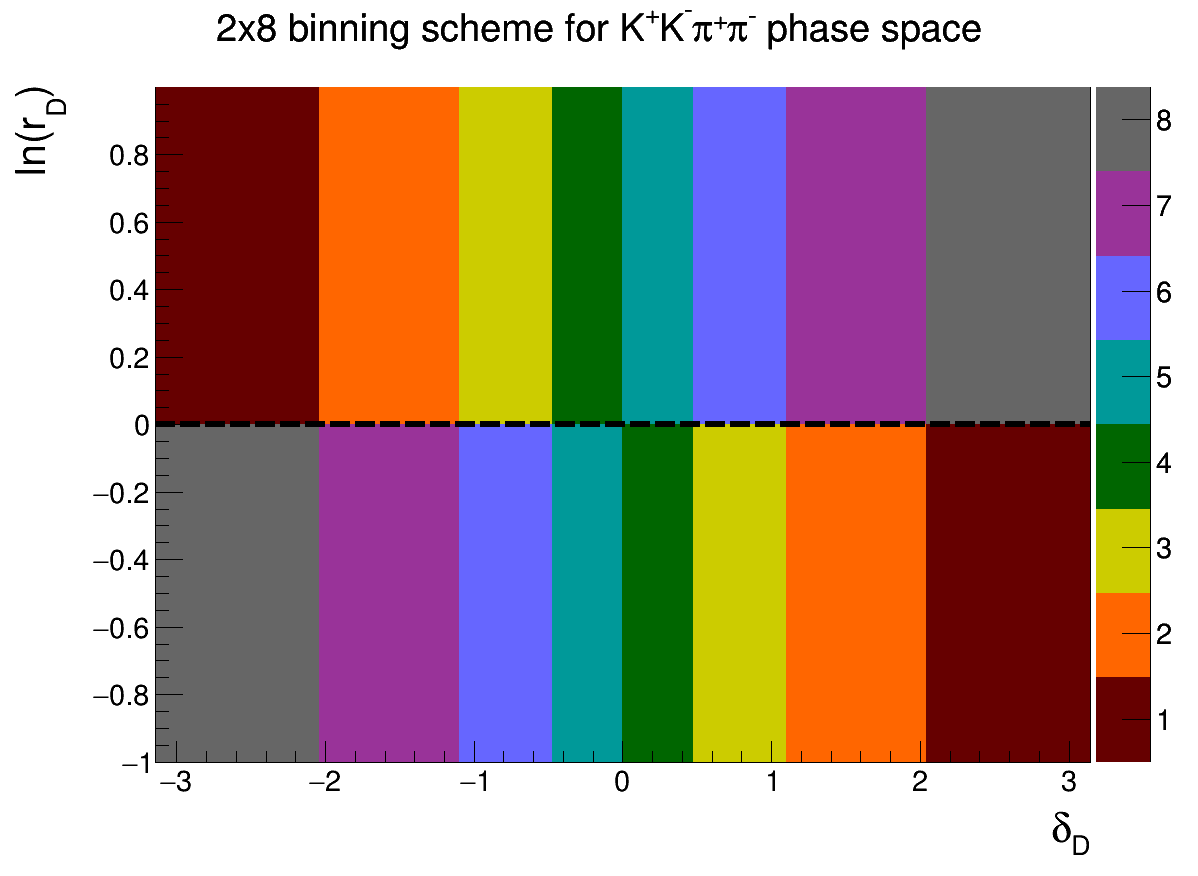
\includegraphics[width=1\textwidth]{Plots/BinningSchemePlot.png}
    \caption{Binning scheme definition for $2\times 8$ bins}
    \label{fig_binning_scheme}
  \end{subfigure}%
  \begin{subfigure}{0.5\textwidth}
    \centering
    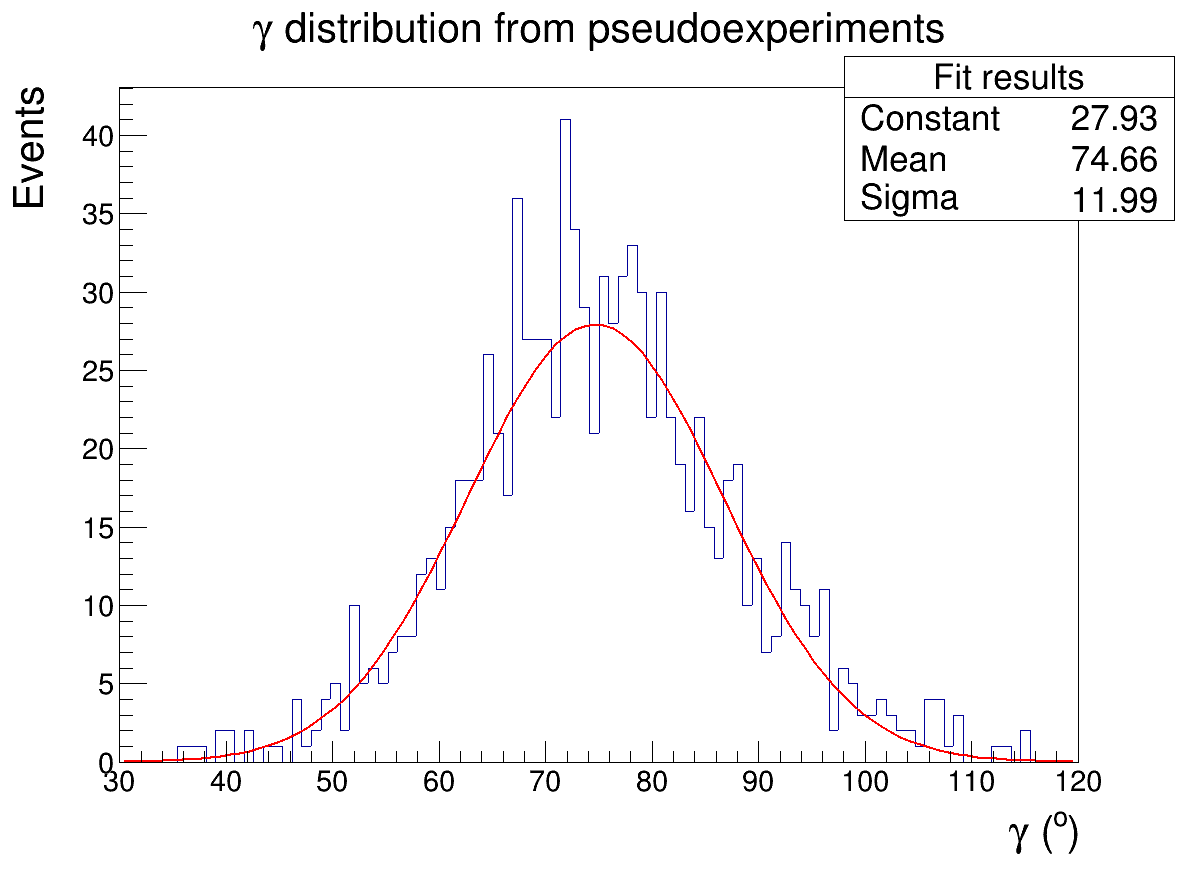
\includegraphics[width=1\textwidth]{Plots/GammaDistribution8BinsVariableWidth.png}
    \caption{Distribution of $\gamma$ from toy study}
    \label{fig_gamma_pull_study}
  \end{subfigure}
  \caption{}
\end{figure}

%%%%%%%%%%%%%%%%%%%%%%%%%%%%%%%%%%%%%%%%%%%%%%%%%%%%%%%%%%%%%%%
\section{\texorpdfstring{$B^\pm$}{B} candidate selection}
\noindent The $B^\pm\to (K^+K^-\pi^+\pi^-)_Dh^\pm (h = \pi, K)$ candidates are reconstructed from five charged tracks. The standard track requirements follow Ref. \cite{cite_LHCbGGSZKSpipi}. A mutually exclusive Particle Identification (PID) cut separates the $B^\pm\to D\pi^\pm$ and $DK^\pm$ candidates. To ensure that $D$ is real, the $K^+K^-\pi^+\pi^-$ invariant mass must be within $\SI{25}{\mega\eV}$ of the $D^0$ mass. Then the tracks are refitted with the $D$ invariant mass constrained and its momentum pointing to the primary vertex. A cut on the $\chi^2$ of this fit removes the $D$ mass sidebands.

$B^\pm\to K^+K^-\pi^+\pi^-h^\pm$ candidates form a charmless background in the $B^\pm$ mass spectrum, but does not peak in the $D$ mass spectrum. To estimate the contamination using data, the $\chi^2$ cut was removed to preserve the $D$ mass sidebands. Inside the mass window $m(K^+K^-\pi^+\pi^-)\in[\SI{1770}{\mega\eV}, \SI{1820}{\mega\eV}]$, a fit to the $B^\pm$ mass spectrum gives a yield of $\SI{2605(57)}{}$. A cut on the flight significance, defined as the flight distance divided by its error, reduces this yield to $\SI{110(19)}{}$. No charmless background was found for $B^\pm\to D\pi^\pm$.

A significant mis-ID background is $B^\pm\to Dh^\pm$, $D\to K^\pm\pi^\mp\pi^\pm\pi^\mp$ and a pion is assigned a kaon hypothesis. A MC simulation sample indicates that $7.2\%$ of $B^\pm$ candidates inside the signal region are $D\to K^\pm\pi^\mp\pi^\pm\pi^\mp$. A tighter PID requirement reduces this this to $1.8\%$ while keeping $93\%$ of signal candidates.

A Boosted Decision Tree (BDT) was used to remove the combinatorial background. The BDT was trained using Monte Carlo (MC) samples as a signal sample and the region $m(Dh^\pm)\in[5800, 7000]\si{\mega\eV}$ in data as a background sample. After training, $99.4\%$ of the combinatorial background was removed and $93\%$ of the signal remained.

%%%%%%%%%%%%%%%%%%%%%%%%%%%%%%%%%%%%%%%%%%%%%%%%%%%%%%%%%%%%%%%
\section{Global fit and invariant mass spectra}
\label{section_global_fit}
\noindent A global ML fit of all $B^\pm\to Dh^\pm (h = K, \pi)$ candidates, shown in Fig. \ref{fig_Bmass_Global}, was performed to determine the yields and shape parameters in the $B^\pm$ mass spectrum, with shape parameterizations from Ref. \cite{cite_LHCbGGSZKSpipi}. Minor adjustments are needed in the final analysis. Currently, only Run $2$ data has been processed, and Run $1$ will be included later.

The combinatorial background is parameterized by an exponential function. The signal is a sum of a Gaussian $f_\text{G}(m|m_B, \sigma)$ and a modified Gaussian,

\begin{equation}
  f_\text{MG}(m|m_B, \sigma, \alpha_L, \alpha_R, \beta)\propto
  \begin{cases}
    \exp\Big(\frac{-\Delta m^2(1 + \beta\Delta m^2)}{2\sigma^2 + \alpha_L\Delta m^2}\Big), \Delta m = m - m_B < 0 \\
    \exp\Big(\frac{-\Delta m^2(1 + \beta\Delta m^2)}{2\sigma^2 + \alpha_R\Delta m^2}\Big), \Delta m = m - m_B > 0 \\
  \end{cases},
\end{equation}
which accounts for the radiated tail and wider resolution. To the left of the $B^\pm$ mass peak are contributions from partially reconstructed backgrounds, where a missing pion or photon leads to peaking at lower mass. These are mainly $B^\pm$ or $B^0$ decays to $Dh^\pm\pi$ or $D^*h^\pm$ with $D^*\to D\pi$ or $D^*\to D\gamma$. Furthermore, in the $B^\pm\to DK^\pm$ channel on the right of the signal, there is a mis-ID component of $B^\pm\to D\pi^\pm$ candidates, where the $\pi^\pm$ is identified as $K^\pm$. This channel also has a component of $B_s\to DK^\pm\pi^\mp$ with a missing pion, and a component of partially reconstructed background from $B^\pm$ and $B^0$ candidates where the $\pi^\pm$ daughter is mis-identified as a $K^\pm$. The fitted yield of $B^\pm\to DK^\pm$ and $B^\pm\to D\pi^\pm$ candidates are $\SI{2290(59)}{}$ and $\SI{33113(211)}{}$, respectively.

\begin{figure}[H] 
  \centering
  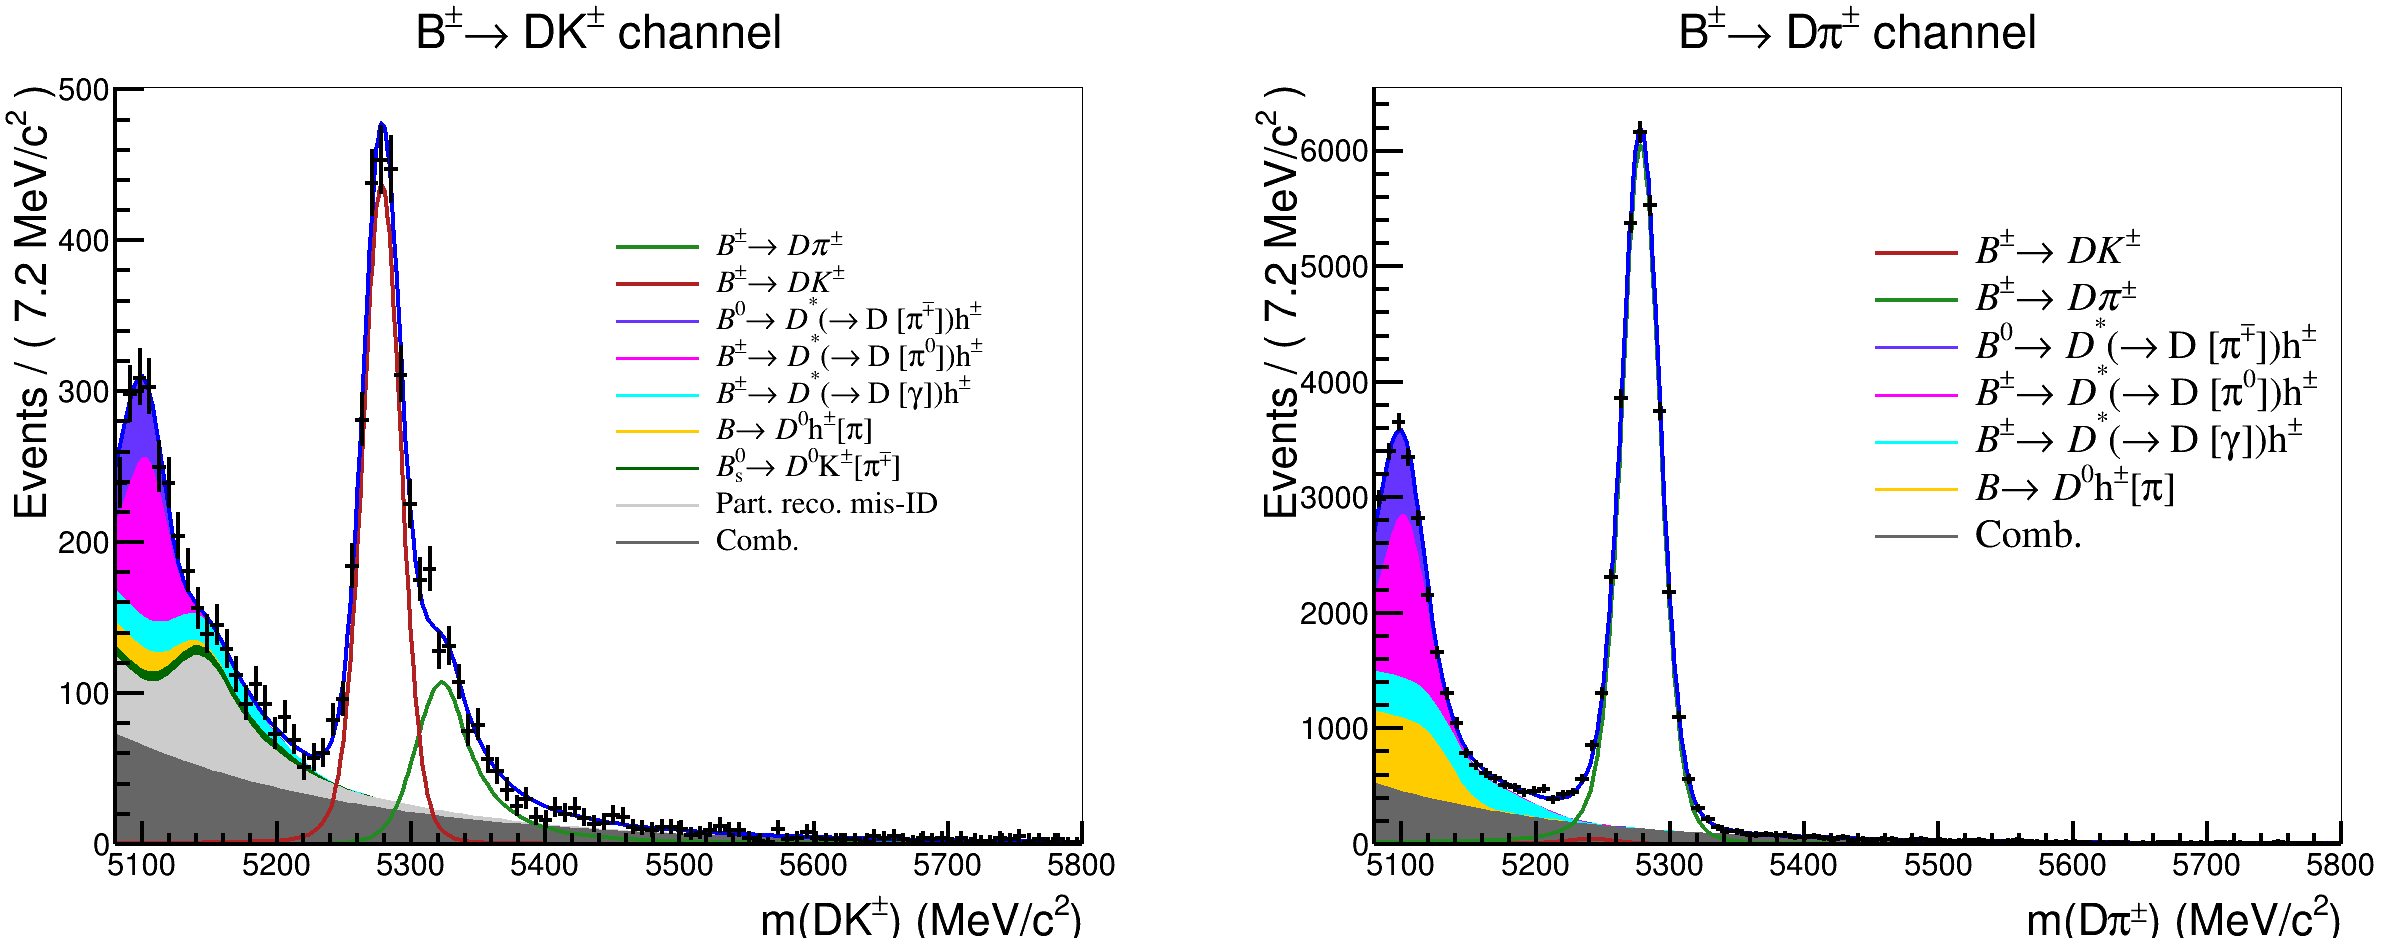
\includegraphics[width=1\textwidth]{Plots/GlobalFit.png}
  \caption{Global mass fit of $B^\pm\to DK^\pm$ (left) and $B^\pm\to D\pi^\pm$ (right).}
  \label{fig_Bmass_Global}
\end{figure}

\section{Binned CP fit and CP observables}
\noindent After the global fit, $B^\pm$ candidates are split by charge and bins, using the binning scheme from Section \ref{section_binning_scheme}. A simultaneous ML fit is performed, with shape parameters from the global fit fixed. The yield of signal, partially reconstructed background and combinatorial background in each bin are floated. The fitted CP observables are shown in Figs. \ref{fig_cp_observables}. Only at the end will these be interpreted in terms of $\gamma$, $\delta_B^{DK}$, $r_B^{DK}$, $\delta^{D\pi}$ and $r_B^{D\pi}$ human bias. Geometrically, the angle between $(x_+^{DK}, y_+^{DK})$ and $(x_-^{DK}, y_-^{DK})$ is $2\gamma$.

To check the fit robustness, $1000$ toy datasets are generated, with both global and binned CP fit, using the fitted parameters. Each toy datasets is then run through the same fitting procecure and the pull distibutions of each floated variable is checked. It was found that all CP observables have pulls with zero mean and unit standard deviation. Two global fit parameters had slightly underestimated errors which can be accounted for.

\begin{figure}[H] 
  \centering
  \begin{subfigure}{0.50\textwidth}
    \centering
    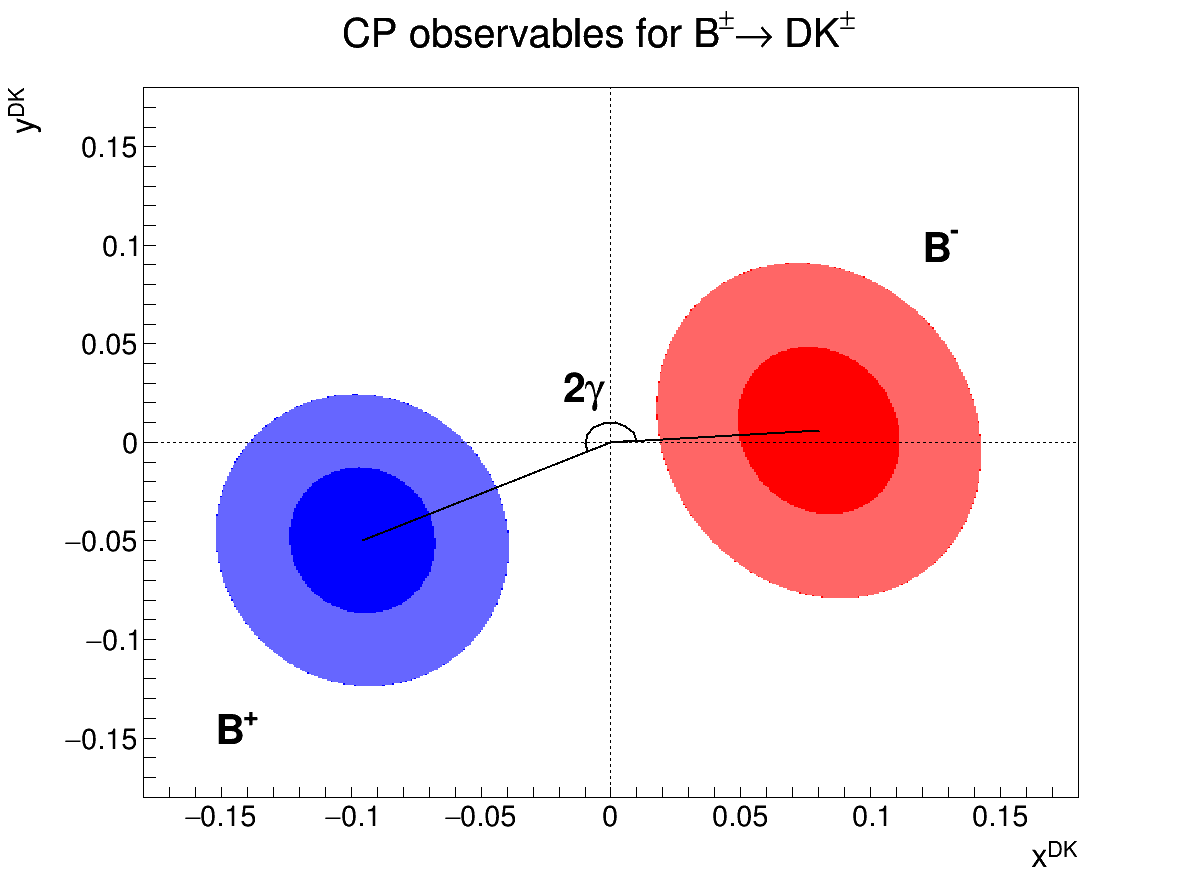
\includegraphics[width=1\textwidth]{Plots/CPContours.png}
  \end{subfigure}%
  \begin{subfigure}{0.50\textwidth}
    \centering
    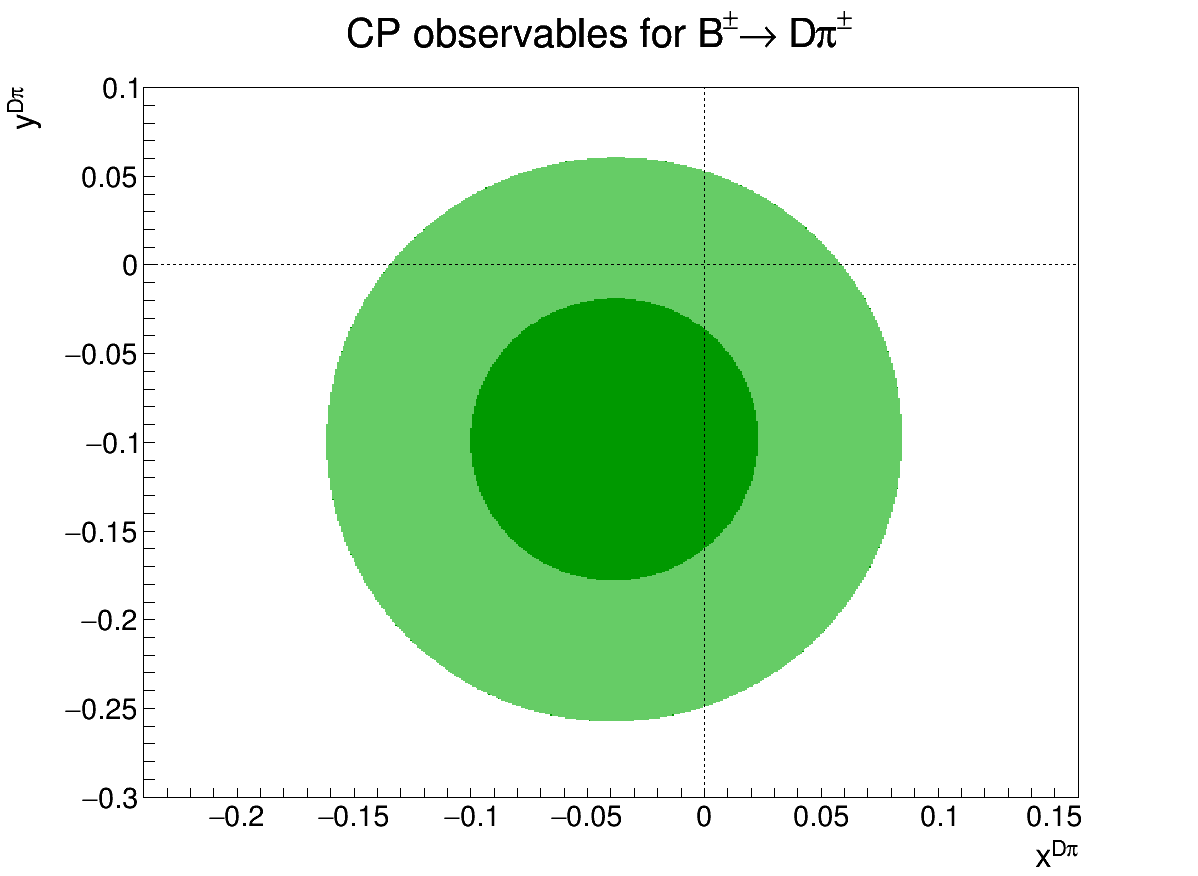
\includegraphics[width=1\textwidth]{Plots/CPXiContours.png}
  \end{subfigure}
  \caption{Confidence levels at $68.2\%$ and $95.5\%$ of $(x_\pm^{DK}, y_\pm^{DK})$ (left) and $(x_\xi^{D\pi}, y_\xi^{D\pi})$ (right).}
  \label{fig_cp_observables}
\end{figure}

%%%%%%%%%%%%%%%%%%%%%%%%%%%%%%%%%%%%%%%%%%%%%%%%%%%%%%%%%%%%%%%
\section{External strong phase input from BESIII}
\noindent The reconstruction of charged and neutral particles follows Ref. \cite{cite_KSKKAnalysis}. For each $D$ meson, beam constrained mass is defined as $M_\text{BC}^2 = E_\text{beam}^2 - \abs{\sum_i\vb{p}_i}^2$. It is the $D$ invariant mass, but using the more accurate beam energy instead of the reconstructed $D$ energy.

The single tag yield is obtained from a ML fit of $M_\text{BC}$. An Argus shape parameterizes the combinatorial background. The signal shape is from a MC sample convolved with a Gaussian. Peaking backgrounds are accounted for with Gaussians. Fig. \ref{fig_styield} shows a fit of $D\to K^+K^-\pi^+\pi^-$. The largest peaking background, in green, is $D\to K_S^0K^+K^-$.

\begin{figure}[H] 
  \centering
  \begin{subfigure}{0.5\textwidth}
    \centering
    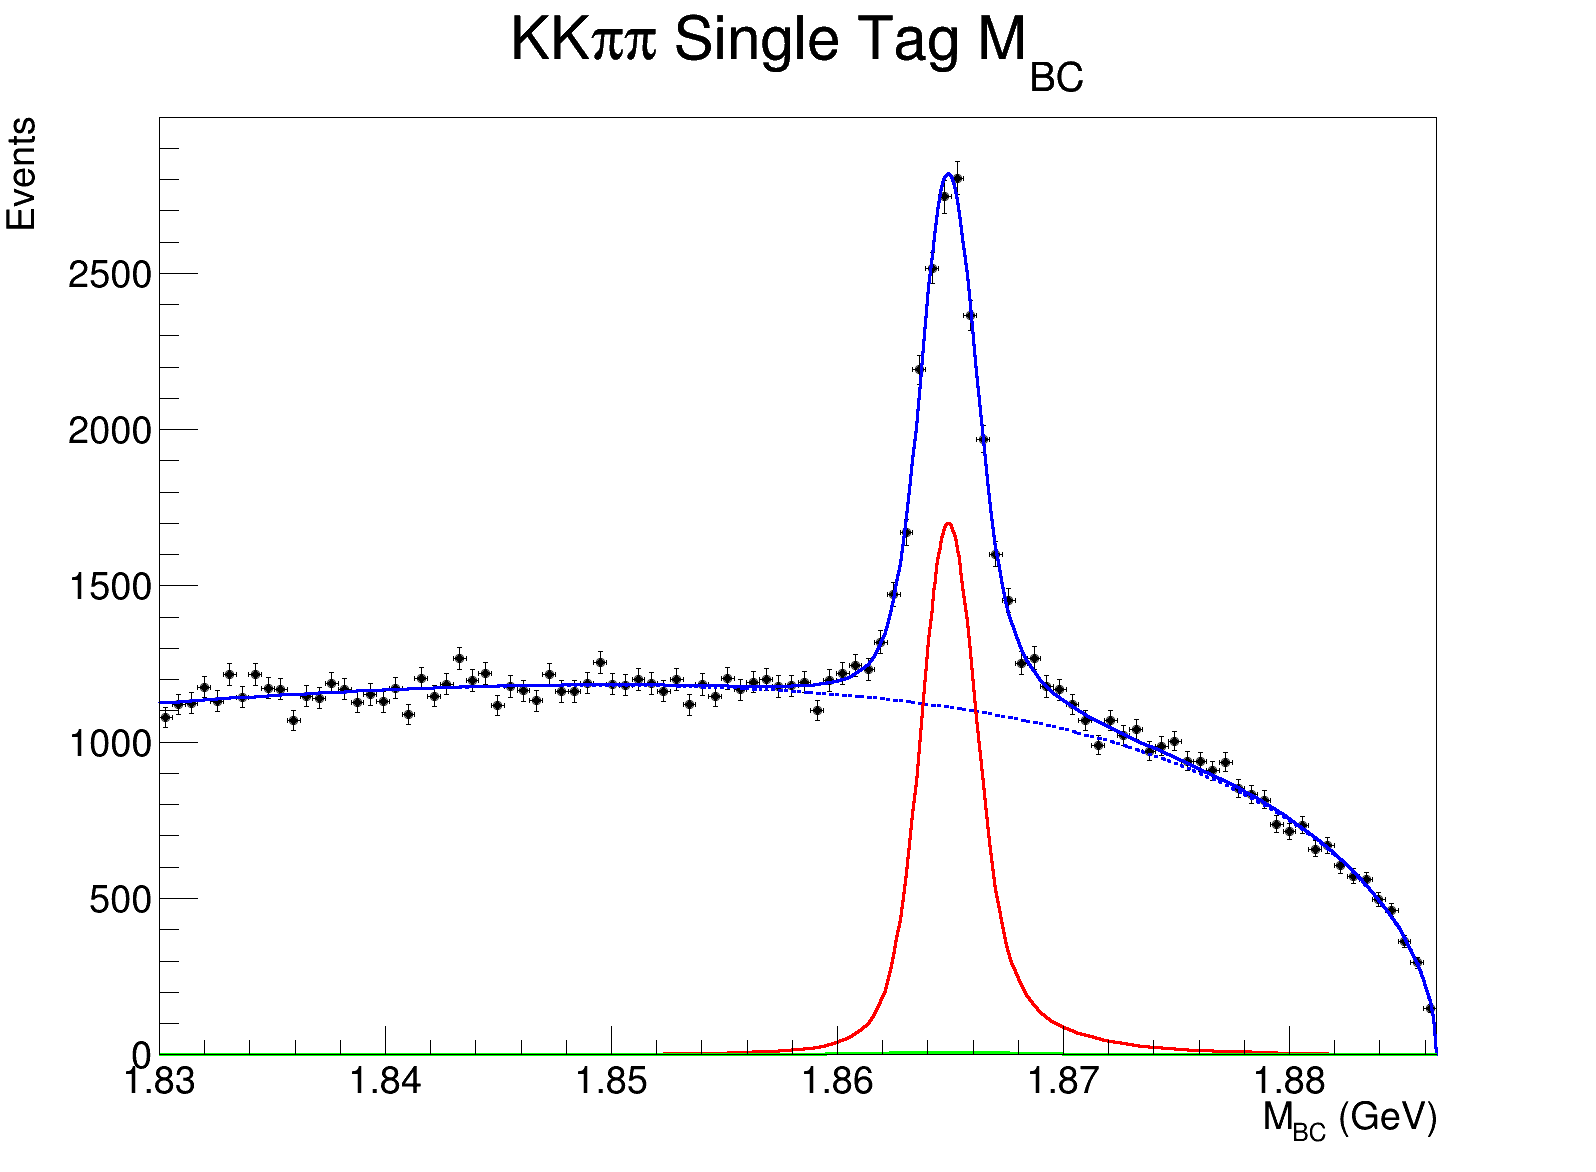
\includegraphics[width=1\textwidth]{Plots/KKpipiSingleTagMBCPlot.png}
    \caption{}
    \label{fig_styield}
  \end{subfigure}%
  \begin{subfigure}{0.5\textwidth}
    \centering
    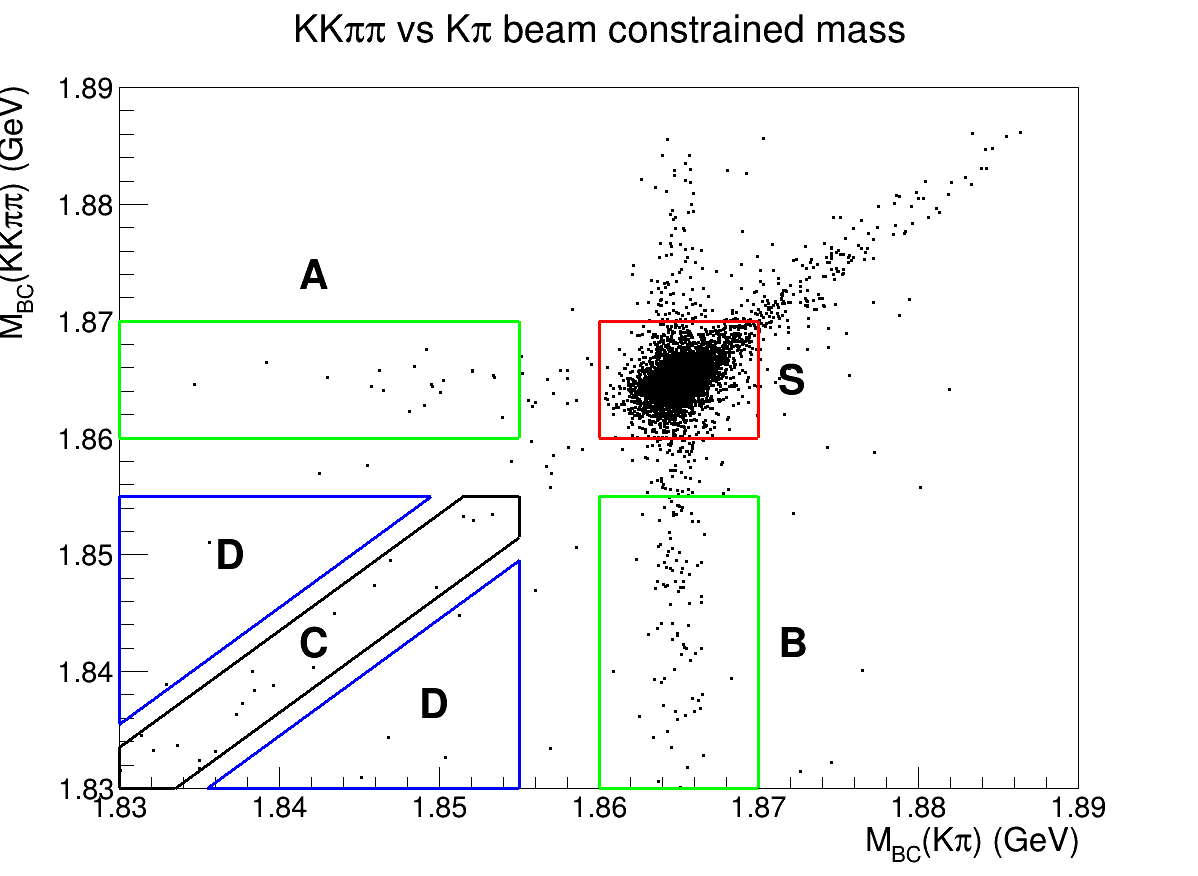
\includegraphics[width=1\textwidth]{Plots/KpiDoubleTagYield.png}
    \caption{}
    \label{fig_dtyield}
  \end{subfigure}
  \caption{Fit of $K^+K^-\pi^+\pi^-$ single tag $M_\text{BC}$ distribution (left) and background subtraction technique of $K^+K^-\pi^+\pi^-$ vs $K^\mp\pi^\pm$ double tag (right).}
\end{figure}

Fig. \ref{fig_dtyield} shows $D\to K^+K^-\pi^+\pi^-$ versus $D\to K^\pm\pi^\mp$ events, where the $M_\text{BC}$ for both $D$ mesons are plotted in a $2$D scatter plot. For double tag yields, a sideband subtraction technique is used. Region $S$ is the signal region, while $A$ and $B$ are events where only one $D$ meson is real. In region $C$ daughters have been swapped between the $D$ mesons. Region $D$ contains non-charm background. The background is estimated using

\begin{equation*}
  B = P + \frac{a_S}{a_D}Y_D + \sum_{i = A, B, C}\frac{a_S}{a_i}\Big(Y_i - \frac{a_i}{A_D}Y_D\Big),
\end{equation*}
where $P$ is the peaking background, and $Y_i$ and $a_i$ are the yield and area of region $i$.

The single and double tag yields are used in a fit of Eqs. \eqref{eq_Mi}-\eqref{eq_Mij} to obtain $c_i$ and $s_i$. Peaking backgrounds are accounted for using inclusive MC samples.

In Fig. \ref{fig_flavour_yield}, $D\to K^\pm\pi^\mp$ vs $D\to K^+K^-\pi^+\pi^-$ events are shown with the LHCb model prediction, using $2\times 4$ bins. Fig. \ref{fig_cp_yield} shows total $D\to K^+K^-\pi^+\pi^-$ event yields, tagged with a CP even and odd modes $D\to K^+K^-$ and $K_S^0\pi^0$. The prediction is normalized by the $K^\pm\pi^\mp$ yields. The data agrees reasonably well with the LHCb model, but the yields have not been corrected for efficiencies and a perfect agreement is therefore not expected.

\begin{figure}[H] 
  \centering
  \begin{subfigure}{0.5\textwidth}
    \centering
    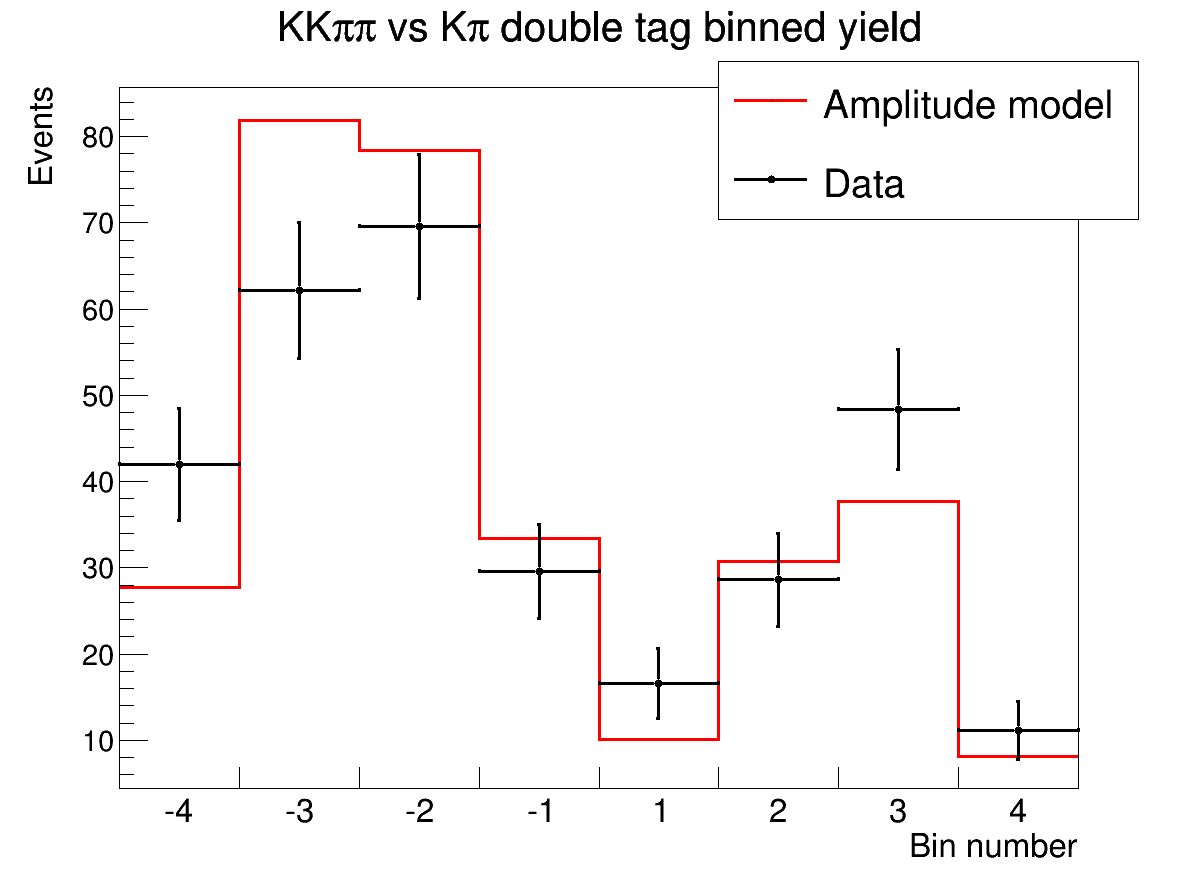
\includegraphics[width=1\textwidth]{Plots/DoubleTagYieldFlavour.png}
    \caption{}
    \label{fig_flavour_yield}
  \end{subfigure}%
  \begin{subfigure}{0.5\textwidth}
    \centering
    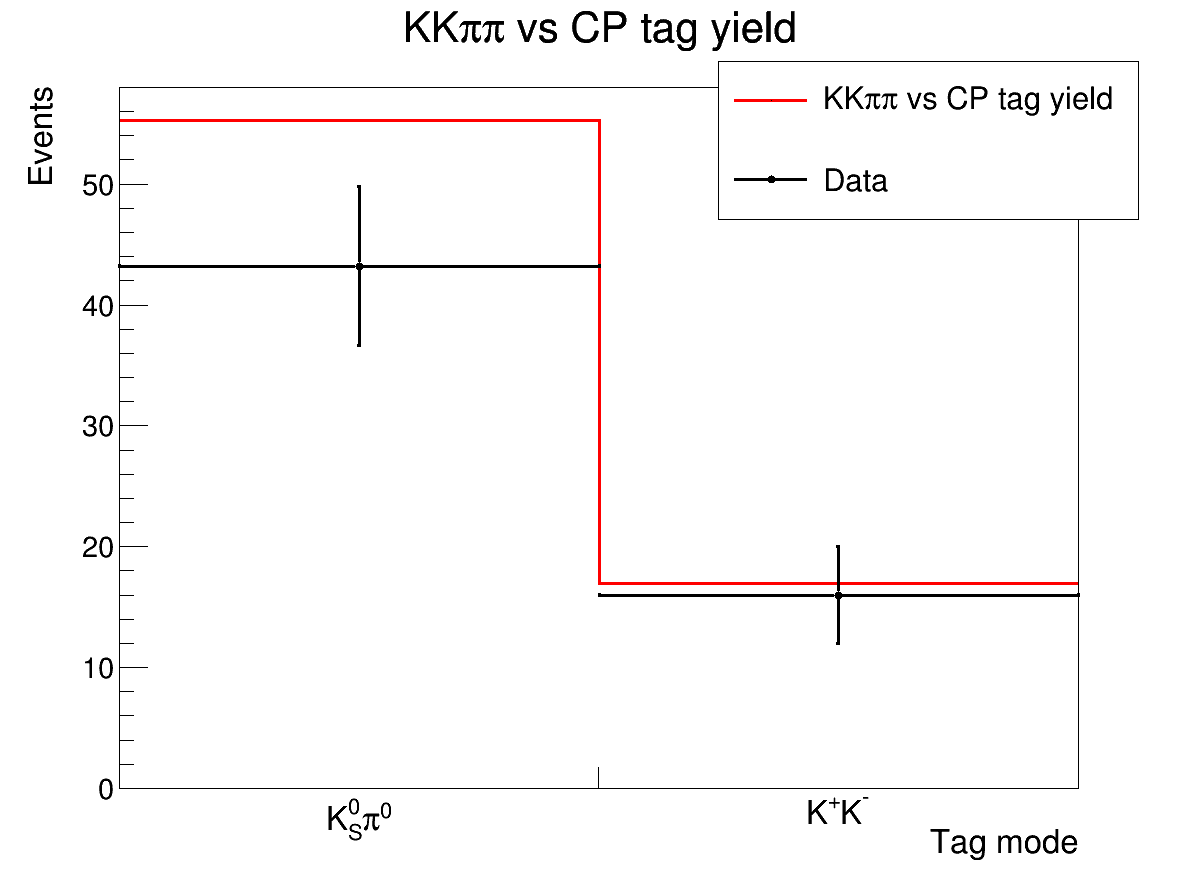
\includegraphics[width=1\textwidth]{Plots/DoubleTagYieldInclusiveCP.png}
    \caption{}
    \label{fig_cp_yield}
  \end{subfigure}
  \caption{Double tag yield of $K^\pm\pi^\mp$ (left), and $K^+K^-$ and $K_S^0\pi^0$ (right).}
\end{figure}

%%%%%%%%%%%%%%%%%%%%%%%%%%%%%%%%%%%%%%%%%%%%%%%%%%%%%%%%%%%%%%%
\section{Conclusion and future work}
\noindent The analysis has so far showed promising results, consistent with prior expectations on both the LHCb and BESIII side. The next steps in the LHCb analysis is optimization of cuts and PDF shape parameters, in addition to a systematics study. For BESIII, the yields and peaking backgrounds of all tag modes must be finalized. Finally, the two analyses will be combined to yield a first measurement of $\gamma$ in this channel.

%%%%%%%%%%%%%%%%%%%%%%%%%%%%%%%%%%%%%%%%%%%%%%%%%%%%%%%%%%%%%%%                                                                          
\bibliography{references}
\bibliographystyle{unsrt}

%%%%%%%%%%%%%%%%%%%%%%%%%%%%%%%%%%%%%%%%%%%%%%%%%%%%%%%%%%%%%%%
\newpage
\section{DPhil thesis plan}
\noindent Discuss DPhil thesis plan with Guy first!

\end{document}